\documentclass[12pt]{article}

\usepackage{sbc-template}
\usepackage[T1]{fontenc}
\usepackage[utf8]{inputenc}
\usepackage[brazil]{babel}
\usepackage{graphicx,url,array}
\urlstyle{same}

\sloppy
\emergencystretch=2em

\title{EduTech Vision: Monitoramento de Atenção, Postura e Engajamento por Processamento Digital de Imagens}

\author{Fernando Cobianchi, Samuel Bernini}

\address{Bacharelado em Ciência da Computação\\
Universidade do Estado de Mato Grosso (UNEMAT)\\
Câmpus Universitário de Rondonópolis -- Rondonópolis -- MT -- Brasil\\
\mbox{}\\[-6pt]\footnotesize\texttt{fernando.cobianchi@unemat.br}\\
\texttt{samuel.bernini@unemat.br}
}

\begin{document}

\maketitle

\begin{abstract}
EduTech Vision is a real-time digital image processing system for educational demonstrations of attention, posture and audience engagement. The current version has individual and audience modes without student identification. The standard pipeline combines OpenCV YuNet, MediaPipe Face Landmarker on expanded crops, EAR/MAR, solvePnP pose, moving averages and 10 s aggregation. In 960x540 smoke benchmarks, enhanced reached F1=0.712/29.0 FPS in individual mode and F1=0.583/74.5 FPS in audience mode. In a 1080p audience audit, it obtained 5/11 exact counts, 10/11 within one face and mean error 0.636. The system is a PDI demonstration, not a pedagogical or clinical diagnostic tool.
\end{abstract}

\begin{resumo}
O EduTech Vision é um sistema de PDI em tempo real para demonstrações educacionais de atenção visual, postura e engajamento. A versão atual opera em modos individual e plateia, sem identificação de estudantes. O pipeline padrão combina OpenCV YuNet, MediaPipe Face Landmarker em recortes ampliados, EAR/MAR, pose por solvePnP, médias móveis e agregação de 10 s. Em benchmarks smoke a 960x540, enhanced alcançou F1=0,712/29,0 FPS no modo individual e F1=0,583/74,5 FPS no modo plateia. Em auditoria 1080p de plateia, obteve 5/11 acertos exatos, 10/11 casos com erro de no máximo um rosto e erro médio 0,636. O sistema é demonstração de PDI, não avaliação pedagógica ou diagnóstico clínico.
\end{resumo}

\section{Introdução}

A observação de atenção, postura e engajamento em ambientes educacionais costuma depender da percepção do professor ou do próprio estudante. Essa percepção é útil, mas é subjetiva, descontínua e difícil de registrar de forma reprodutível. Em projetos de Processamento Digital de Imagens (PDI), sinais visuais como abertura dos olhos, abertura da boca, orientação da cabeça e presença de faces podem ser utilizados para demonstrar como medidas geométricas e temporais transformam imagens em indicadores aproximados.

Neste contexto, o EduTech Vision foi desenvolvido como produto acadêmico da Trilha 3: Atenção, Postura e Engajamento. O sistema possui dois cenários complementares: no modo individual, uma câmera frontal acompanha uma pessoa e estima fadiga, bocejo, queda postural e desatenção sustentada; no modo plateia, uma câmera voltada a um grupo calcula métricas agregadas de faces voltadas ao palco ou professor. O modo plateia não identifica alunos e não produz decisões individualizadas.

O objetivo deste artigo é apresentar a versão atual do sistema com linguagem científica e evidências compatíveis com os resultados atuais disponíveis. O trabalho não afirma medir aprendizagem, rendimento escolar ou estado clínico. Os indicadores gerados são aproximações visuais para fins de demonstração acadêmica de PDI em tempo real.

\section{Fundamentação}

PDI e visão computacional combinam aquisição, pré-processamento, extração de características e tomada de decisão para interpretar padrões visuais \cite{gonzalez2018,szeliski2022}. Em aplicações com faces, detectores localizam regiões de interesse, enquanto modelos de landmarks estimam pontos anatômicos que permitem calcular medidas geométricas. O uso de detectores pré-treinados como front-end é adequado quando o processamento posterior explicita o núcleo de PDI, como ocorre com razões geométricas, estimativa de pose e suavização temporal.

No modo individual, a razão de aspecto dos olhos, ou Eye Aspect Ratio (EAR), é calculada pela razão entre distâncias verticais e horizontais de pontos das pálpebras. Reduções sustentadas do EAR indicam olhos fechados por mais tempo que uma piscada comum. De modo análogo, a Mouth Aspect Ratio (MAR) relaciona abertura vertical e largura da boca, permitindo sinalizar bocejo quando o valor permanece elevado. Essas métricas são sensíveis a escala, pose, iluminação e qualidade dos landmarks; por isso são suavizadas antes da decisão.

A postura e o foco visual aproximado são estimados por pose de cabeça. O sistema usa correspondências 2D-3D de pontos faciais e a função solvePnP para obter yaw, pitch e roll. No modo plateia, yaw e pitch são comparados a um eixo de referência calibrado no início da sessão. A decisão final é agregada em janela temporal, pois quadros isolados podem conter ruído, oclusões ou landmarks incompletos.

\section{Sistema Proposto}

A Figura~\ref{fig:pipeline} sintetiza o pipeline atual. A entrada pode ser câmera ou vídeo, processada em resolução padrão de 960x540. O perfil padrão é enhanced: OpenCV YuNet detecta faces, aplica supressão de não máximos e prioriza candidatos; em seguida, cada região é recortada com margem ampliada e enviada ao MediaPipe Face Landmarker. O perfil mediapipe é mantido como baseline, enquanto o perfil research, baseado em SCRFD, é apenas comparativo acadêmico e não constitui o padrão de distribuição.

\begin{figure}[!htbp]
\centering
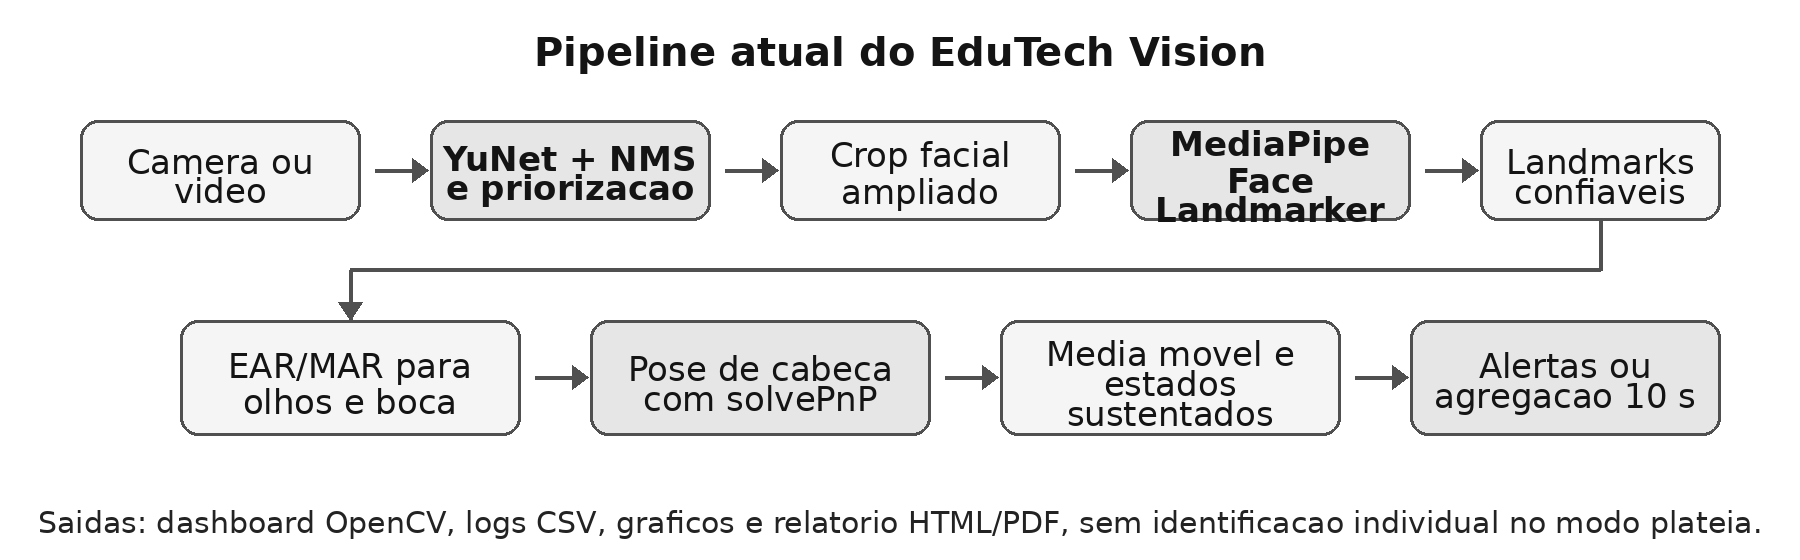
\includegraphics[width=\textwidth]{pipeline_original.png}
\caption{Pipeline atual do EduTech Vision.}
\label{fig:pipeline}
\end{figure}

No modo individual, a configuração atual usa confiança facial 0,70 e no máximo uma face. A primeira etapa de uso realiza calibração de 5 s para estabelecer referências de EAR, MAR, yaw e pitch. Em seguida, as medidas passam por média móvel de janela 7 e por condições sustentadas, evitando que piscadas ou movimentos pontuais acionem alertas. Os alertas visuais indicam fadiga, bocejo, postura ruim e desatenção, sem atribuir diagnóstico clínico.

No modo plateia, a configuração atual usa confiança facial 0,60, limite de 24 faces, tolerância de 30 graus em yaw, tolerância de 20 graus em pitch e janela de agregação de 10 s. Faces detectadas sem landmarks confiáveis podem aparecer no painel visual como detecções anônimas, mas não entram no cálculo de pose e engajamento. A saída persistida é agregada, composta por séries temporais e estatísticas da sessão.

\section{Metodologia Experimental}

A avaliação foi organizada em quatro frentes. A primeira é o benchmark smoke do detector, que compara o baseline MediaPipe em quadro inteiro com o perfil enhanced em dois modos. As métricas são recall de face, recall de landmarks, precisão, F1, FPS médio e FPS mínimo. O recall de face considera uma caixa localizada corretamente; o recall de landmarks é mais restritivo e exige que a face também gere pontos suficientes para EAR, MAR ou pose.

A segunda frente é a auditoria HQ de plateia. Nessa avaliação, vídeos 1080p são processados integralmente e quadros selecionados são comparados com contagens manuais de rostos avaliáveis. As métricas são acertos exatos, casos com erro de no máximo um rosto, erro absoluto médio, presença da contagem manual dentro da janela temporal de mais ou menos 1 s, FPS médio e FPS no percentil 10.

A terceira frente é o relatório de sessão. Ele demonstra instrumentação da aplicação por meio de logs CSV, gráficos, relatório HTML, relatório PDF, timeline de eventos e telemetria. Esses artefatos são usados para evidenciar capacidade de registro e reprodutibilidade da demonstração, e não como verdade final dos protocolos formais.

Por fim, a versão atual contém metodologia e scripts para os cinco protocolos formais do plano da disciplina: robustez luminosa, resiliência a oclusão, telemetria de FPS, matriz de confusão e tolerância a falhas. Entretanto, não foram usados resultados históricos, preliminares ou logs finais antigos como evidência da versão atual. Na ausência de novos registros experimentais finais desses cinco protocolos, eles são tratados neste artigo como metodologia disponível para reexecução. O suporte a reconexão de câmera é descrito apenas como característica de robustez implementada, não como resultado experimental principal.

\section{Resultados}

A Tabela~\ref{tab:benchmark} apresenta o benchmark smoke canônico da versão atual. Em ambos os modos, o perfil enhanced aumenta substancialmente o recall de face e o F1 em relação ao baseline MediaPipe, mantendo desempenho em tempo real. A redução de FPS é esperada, pois o pipeline passa a executar detecção por YuNet, recortes ampliados e landmarks em regiões de interesse, em vez de depender apenas do rastreamento direto no quadro inteiro.

\begin{table}[!htbp]
\centering
\caption{Benchmark smoke do detector em 960x540.}
\label{tab:benchmark}
\scriptsize
\begin{tabular}{|c|c|c|c|c|c|c|c|}
\hline
\textbf{Modo} & \textbf{Perfil} & \textbf{Recall face} & \textbf{Recall landmarks} & \textbf{Precisão} & \textbf{F1} & \textbf{FPS médio} & \textbf{FPS mín.}\\
\hline
Individual & mediapipe & 0,193 & 0,193 & 1,000 & 0,324 & 242,4 & 91,7\\
\hline
Individual & enhanced & 0,592 & 0,294 & 0,894 & 0,712 & 29,0 & 19,3\\
\hline
Plateia & mediapipe & 0,011 & 0,011 & 1,000 & 0,022 & 491,6 & 154,6\\
\hline
Plateia & enhanced & 0,443 & 0,089 & 0,851 & 0,583 & 74,5 & 56,3\\
\hline
\end{tabular}
\end{table}

A Tabela~\ref{tab:auditoria} resume a auditoria HQ do modo plateia com a configuração enhanced, confiança 0,60 e limite de 24 faces. Diferentemente da Tabela~\ref{tab:benchmark}, essa avaliação usa vídeos 1080p completos, cenas mais pesadas e comparação com contagem manual em quadros específicos. Portanto, o FPS dessa auditoria não deve ser comparado diretamente com o FPS do benchmark de detector em 960x540.

\begin{table}[!htbp]
\centering
\caption{Auditoria HQ de plateia com configuração enhanced, confiança 0,60 e limite de 24 faces.}
\label{tab:auditoria}
\small
\begin{tabular}{|p{6.8cm}|p{4.2cm}|}
\hline
\textbf{Métrica} & \textbf{Resultado}\\
\hline
Acertos exatos & 5/11\\
\hline
Erro de no máximo 1 rosto & 10/11\\
\hline
Erro absoluto médio & 0,636 rosto\\
\hline
Manual dentro da janela +/-1 s & 10/11\\
\hline
FPS médio & 13,3\\
\hline
FPS p10 & 9,4\\
\hline
\end{tabular}
\end{table}

A matriz de confusão disponível na versão revisada é demonstrativa. Ela contém 50 amostras sintéticas de atenção e desatenção, usadas para testar o fluxo de cálculo, visualização e relatório. A Tabela~\ref{tab:confusao} mostra que houve 46 acertos e 4 erros, produzindo acurácia, precisão macro, recall macro e F1 macro de 0,92. Como as amostras são explicitamente demonstrativas, esse resultado não é apresentado como validação científica real; a validação final exige amostras reais rotuladas.

\begin{table}[!htbp]
\centering
\caption{Matriz de confusão demonstrativa com 50 amostras.}
\label{tab:confusao}
\small
\begin{tabular}{|c|c|c|}
\hline
\textbf{Classe real} & \textbf{Predito atento} & \textbf{Predito desatento}\\
\hline
Atento & 23 & 2\\
\hline
Desatento & 2 & 23\\
\hline
\end{tabular}
\end{table}

O relatório de sessão demonstra que a aplicação gera CSVs de telemetria, gráficos, páginas HTML, PDF e linha do tempo de eventos. Seus valores numéricos não foram usados para substituir a reexecução formal dos cinco protocolos, mas comprovam que o sistema está instrumentado para registrar sessões e produzir artefatos analisáveis.

\section{Discussão}

Os resultados justificam o uso do perfil enhanced como padrão. O baseline MediaPipe é muito rápido, mas perde muitas faces pequenas ou distantes, sobretudo no modo plateia. O uso de YuNet antes dos landmarks aumenta o recall de faces e torna a interface mais útil para demonstrações com mais de uma pessoa. A principal contrapartida é a queda de FPS e a diferença entre detecção de face e disponibilidade de landmarks.

Essa diferença é importante para interpretar o sistema. Uma face pode ser localizada por caixa, mas não gerar landmarks estáveis o suficiente para pose, EAR ou MAR. Nesses casos, a face pode ser desenhada de forma anônima, mas não deve influenciar métricas de atenção ou engajamento. Por isso, recall de face e recall de landmarks são relatados separadamente.

Também há diferença metodológica entre o FPS do benchmark e o FPS da auditoria HQ. O benchmark smoke mede o pipeline do detector em 960x540, com foco em comparação controlada entre perfis. A auditoria HQ processa vídeos 1080p completos, registra respostas por frame e avalia cenas com maior densidade visual. É esperado que os valores absolutos de FPS sejam menores nesse contexto.

As limitações observadas são coerentes com aplicações de visão computacional em tempo real. Iluminação irregular, distância da câmera, oclusão parcial, rostos em perfil, faces pequenas, motion blur e cortes nas bordas reduzem a estabilidade dos landmarks. No modo individual, EAR e MAR variam entre pessoas e dependem da calibração inicial. No modo plateia, a métrica agregada estima orientação visual aproximada e não atenção cognitiva ou aprendizagem.

\section{Considerações Éticas e LGPD}

O EduTech Vision trata imagem de pessoas e, portanto, deve ser usado com minimização de dados, transparência e finalidade acadêmica. No modo individual, a captura deve ocorrer com consentimento do participante e sem uso punitivo, clínico ou classificatório. No modo plateia, o sistema opera apenas com métricas agregadas e não deve identificar alunos, registrar nomes, persistir frames ou permitir reidentificação.

Por padrão, a proposta privilegia processamento local, descarte de imagens e armazenamento apenas de séries temporais, contagens, percentuais agregados e eventos de interface. Relatórios e gráficos devem ser usados para explicar o comportamento do pipeline, não para vigiar indivíduos. Em demonstrações públicas, recomenda-se sinalização visível sobre a captura de imagem, opção de afastamento da câmera e uso de voluntários quando forem necessárias evidências visuais.

Essas escolhas atendem ao princípio de necessidade da Lei Geral de Proteção de Dados e reduzem o risco de interpretação abusiva. O sistema deve ser entendido como material didático de PDI, não como tecnologia de decisão automatizada sobre estudantes.

\section{Conclusão}

Este artigo apresentou a versão atual do EduTech Vision, uma aplicação funcional de PDI em tempo real para monitoramento aproximado de atenção visual, postura e engajamento agregado. A arquitetura atual combina YuNet, MediaPipe Face Landmarker em recortes ampliados, EAR, MAR, solvePnP, suavização temporal e relatórios de sessão. O benchmark smoke mostra que o perfil enhanced supera o baseline MediaPipe em recall e F1 nos dois modos, enquanto a auditoria HQ indica desempenho aceitável para contagem agregada em vídeos mais pesados.

As evidências atuais sustentam o sistema como demonstração reprodutível e tecnicamente coerente para a Trilha 3. Ao mesmo tempo, a matriz de confusão disponível é apenas demonstrativa e os cinco protocolos formais devem ser reexecutados com novos registros experimentais finais para uma validação máxima da versão atual. Trabalhos futuros incluem ampliar amostras reais rotuladas, testar diferentes condições de iluminação e distância, melhorar a estabilidade de landmarks em rostos pequenos e refinar a comunicação ética do uso em ambientes educacionais.

\section*{Agradecimentos}

Os autores agradecem ao curso de Bacharelado em Ciência da Computação da UNEMAT e ao docente da disciplina de Processamento Digital de Imagens pelas diretrizes do projeto. Ferramentas de IA generativa foram utilizadas pontualmente como apoio à revisão gramatical e à organização textual; o conteúdo técnico, a interpretação dos resultados e a responsabilidade final permanecem dos autores.

\begingroup
\raggedright
\begin{thebibliography}{}

\bibitem[Brasil 2018]{brasil2018}
Brasil (2018). Lei n\textsuperscript{o} 13.709, de 14 de agosto de 2018. Lei Geral de Proteção de Dados Pessoais.

\bibitem[Gonzalez and Woods 2018]{gonzalez2018}
Gonzalez, R. C. and Woods, R. E. (2018). Processamento Digital de Imagens. 4. ed. Pearson.

\bibitem[Google 2026]{google2026}
Google (2026). MediaPipe Face Landmarker. Disponível em: \url{https://developers.google.com/mediapipe}. Acesso em: 2026.

\bibitem[OpenCV 2026]{opencv2026}
OpenCV (2026). OpenCV Documentation. Disponível em: \url{https://docs.opencv.org}. Acesso em: 2026.

\bibitem[OpenCV Zoo 2026]{opencvzoo2026}
OpenCV Zoo (2026). YuNet Face Detection. Disponível em: \url{https://github.com/opencv/opencv_zoo/tree/main/models/face_detection_yunet}. Acesso em: 2026.

\bibitem[Szeliski 2022]{szeliski2022}
Szeliski, R. (2022). Computer Vision: Algorithms and Applications. 2. ed. Springer.

\bibitem[Yang et al. 2016]{yang2016}
Yang, S., Luo, P., Loy, C. C. and Tang, X. (2016). WIDER FACE: A Face Detection Benchmark. In Proceedings of the IEEE Conference on Computer Vision and Pattern Recognition.

\end{thebibliography}
\endgroup

\end{document}
